\documentclass{beamer}

\usepackage[utf8]{inputenc}
\usepackage[T1]{fontenc}

\usepackage[english]{babel}
\usepackage{amsmath}
\usepackage{cleveref}
\usepackage{amssymb}
\usepackage{mathtools}

%%Numbers, expectation
\newcommand{\N}{\mathbb{N}}
\newcommand{\E}{\mathbb{E}}
\renewcommand{\P}{\mathbb{P}}
\newcommand{\Var}{\mathbb{V}}
\newcommand{\R}{\mathbb{R}}
\newcommand{\D}{\mathcal{D}}
\newcommand{\B}{\mathcal{B}}
\newcommand{\Dh}{\D_h}
\renewcommand{\phi}{\varphi}
\newcommand*\diff{\mathop{}\!\mathrm{d}} % integral

%% mathoperator
\DeclareMathOperator*{\argmax}{arg\,max}
\DeclareMathOperator*{\argmin}{arg\,min}
\DeclareMathOperator*{\dom}{dom}
\DeclareMathOperator*{\sign}{sign}
\DeclareMathOperator*{\diag}{diag}

\DeclareMathOperator*{\Cov}{Cov}
\DeclareMathOperator*{\Cor}{Corr}
\DeclareMathOperator*{\Id}{Id}

%proximal operator
\newcommand{\prox}[3][]{\operatorname{prox}^{#1}_{#2}\left(#3 \right)}

\usepackage{xcolor}

%% sort citations by increasing number
\usepackage[sort,nocompress]{cite}

\usepackage{graphicx}% http://ctan.org/pkg/graphicx
\graphicspath{{../figures/}{../../figures}{../../memes}} %Setting the graphicspath
\usepackage{caption,subcaption}

\usepackage{tikz}
\usepackage{pgfplots}
\usetikzlibrary{backgrounds}
\usetikzlibrary{intersections}
\usepgfplotslibrary{fillbetween}

% \usepackage[right]{showlabels}


%%
\theoremstyle{plain}
\newtheorem{prop}{Proposition}[section]
\newtheorem{algo}{Algorithm}[section]
\newtheorem{assumption}{Assumption}
\theoremstyle{remark}
\newtheorem{remark}{Remark}[section]

% cref
\crefname{assumption}{Assumption}{Assumptions}
\crefname{equation}{}{}

\usepackage{autonum}

\usepackage{bm} %% bold math symbols

\usepackage{bbm} %% for \mathbbm{1}


% algorithmic environment
\usepackage{algorithm}
\usepackage[noend]{algpseudocode}

% for some reason this was required on one void linux installation (but not the other)
\usepackage{sansmathaccent}
\pdfmapfile{+sansmathaccent.map}

\author{Axel Böhm}

% shows which section we're in
\usetheme{Darmstadt}

% page number
\setbeamertemplate{footline}[frame number]
\setbeamercolor{page number in head/foot}{fg=gray}


% display things like onslide or visible already before but grayed out
\setbeamercovered{transparent}

% set the itemize item symbol as a diamond
\setbeamertemplate{itemize item}{$\diamond$}
% set the itemize subitem symbol as a triangle
\setbeamertemplate{itemize subitem}{$\blacktriangleright$}

% set the enumerate item symbol as a roman numbers
\setbeamertemplate{enumerate item}{(\roman{enumi})}


\title{Matrix scaling}
\date{\today}

\begin{document}
\maketitle
\frame{\tableofcontents[currentsection]}

\section{Introduction}%

\begin{frame}
  \frametitle{Introduction}
  \textbf{given:} a matrix $A \in \R^{m\times n}_+$, vectors $r \in \R_{++}^m$ and $c \in \R^n_{++}$\\
  \textbf{find:} diagonal matrices $X$ and $Y$ such that for $B = XAY$ it holds:
  \begin{equation}
    B \mathbbm{1}_n = r \quad \text{and} \quad B^T \mathbbm{1}_m = c
  \end{equation}
  where $\mathbbm{1}_n = (1, \dots, 1)$ exactly $n$-times.
  Equivalently
  \begin{equation}
    \Vert B_{i,:} \Vert_1 = r_i \quad \text{and} \Vert B_{:, j} \Vert = c_j.
  \end{equation}

  \begin{block}{}
    In this case $A$ is called $(r,c)$-scalable.
  \end{block}
  \onslide<2->{%
    If $\Vert r \Vert_1 \neq \Vert c \Vert_2$ this is not possible.
  }
\end{frame}

\begin{frame}
  \frametitle{Visualization of diagonal scaling}

  \begin{equation}
    \begin{aligned}
    B = \begin{bmatrix}
      x_1 & & & \\
      & x_2 & & \\
      & & \ddots & \\
      & & & x_m
    \end{bmatrix}
    A
    \begin{bmatrix}
      y_1 & & & \\
      & y_2 & & \\
      & & \ddots & \\
      & & & y_n
    \end{bmatrix}
    \\
    =
    \begin{bmatrix}
      a_{1,1}x_1y_1 & a_{1,2}x_1y_2 & \cdots & a_{1,n} x_1y_m \\
      \vdots   & \ddots & & \\
      a_{m,1}x_m y_1 & & \cdots & a_{m,n}x_m y_m
    \end{bmatrix}
    \end{aligned}
  \end{equation}
\end{frame}


\begin{frame}
  \frametitle{Applications}
  \begin{block}{Ill conditioned linear system $Az = b$.}
    Can multiply both sides by $X$  and substitute $z= Yv$ to get instead
    \begin{equation}
      XAz = X
    \end{equation}
  \end{block}
  \begin{block}{$(0-1)$ matrices | bipartite graphs}
  \end{block}
  \begin{minipage}{0.5\textwidth}
    \begin{equation}
      \begin{bmatrix}
        0 & 1 & 1 \\
        1 & 0 & 0 \\
        0 & 1 & 1
      \end{bmatrix}
    \end{equation}
  \end{minipage}
  \begin{minipage}{0.25\textwidth}
    \begin{figure}[ht]
      \centering
      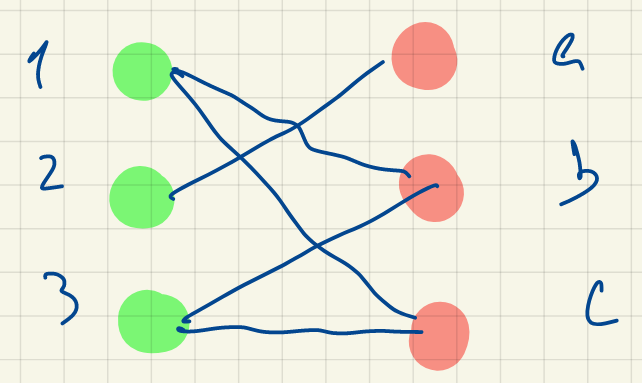
\includegraphics[width=\textwidth]{bipartite-graph.png}
      \caption{\label{fig:label} }
    \end{figure}
  \end{minipage}
  \begin{definition}
    A \textbf{matching} is a set of edges without common vertices.
  \end{definition}
  \begin{definition}
    A \textbf{perfect matching} is a matching which covers all vertices.
  \end{definition}






\end{frame}

\end{document}
